% !TEX program = xelatex
% ============================================================================
%  2025—2026 学年度第二学期高二年级期末教学质量监测试卷 · 数学
%  排版参照真实高考试卷样式（原卷 + 参考答案分离）
% ============================================================================
\documentclass[a4paper,12pt]{ctexart}

% ==================== 宏包 ====================
\usepackage[top=2.2cm,bottom=2.2cm,left=2.5cm,right=2.5cm]{geometry}
\usepackage{amsmath,amssymb}
\usepackage{bm}
\usepackage{graphicx}
\usepackage{float}
\usepackage{enumitem}
\usepackage{multicol}
\usepackage{tabularx}
\usepackage{multirow}
\usepackage{booktabs}
\usepackage{fancyhdr}
\usepackage{xcolor}
\usepackage{titlesec}
\usepackage{caption}
\usepackage{setspace}
\usepackage{framed}

% ==================== 页面样式 ====================
% 试卷部分的"共?页"手动指定（编译后根据实际页数修改）
\newcommand{\questiontotalpages}{4}

\pagestyle{fancy}
\fancyhf{}
\renewcommand{\headrulewidth}{0pt}
\renewcommand{\footrulewidth}{0.4pt}



% 首页样式
\fancypagestyle{firstpage}{
  \fancyhf{}
  \renewcommand{\headrulewidth}{0pt}
  \renewcommand{\footrulewidth}{0.4pt}

}

% 答案页样式（带页眉）
\fancypagestyle{answerstyle}{
  \fancyhf{}
  \renewcommand{\headrulewidth}{0.4pt}
  \renewcommand{\footrulewidth}{0.4pt}

}

% ==================== 标题格式 ====================
\titleformat{\section}[hang]{\centering\zihao{4}\heiti}{}{0em}{}
\titlespacing{\section}{0pt}{0pt}{4pt}

% ==================== 列表设置 ====================
\setlist{nosep,leftmargin=*}

% ==================== 正文行距 ====================
\onehalfspacing

\begin{document}

% ==================== 试 卷 部 分 ====================
% （试卷最后一页的引用标签在答案部分之前定义）

% ---------- 第1页 ----------
\thispagestyle{firstpage}

% 顶部左右信息
\begin{minipage}[t]{0.48\textwidth}
  \zihao{-5}\heiti 绝密$\bigstar$启用前
\end{minipage}
\hfill
\begin{minipage}[t]{0.48\textwidth}
  \raggedleft\zihao{-5}\heiti 试卷类型：A
\end{minipage}

\vspace{0.3cm}

% 标题
\begin{center}
{\zihao{4}\heiti 2025---2026 学年度第二学期高二年级期末教学质量监测试卷}\\[0.4em]
{\zihao{-1}\heiti\bfseries 数 \quad 学}
\end{center}

\vspace{0.3cm}

% 注意事项
{\heiti\zihao{5} 注意事项：}
\begin{enumerate}[label=\arabic*.,leftmargin=2em,itemsep=1pt,topsep=2pt]
  \item 考生答卷前，务必将自己的姓名、座位号写在答题卡上。将条形码粘贴在规定区域。本试卷满分 \textbf{150} 分，考试时间 \textbf{120} 分钟。
  \item 做选择题时，选出每小题答案后，用铅笔把答题卡上对应题目的答案标号涂黑。如需改动，用橡皮擦干净后，再选涂其他答案标号。写在本试卷上无效。
  \item 回答非选择题时，将答案写在答题卡的规定区域内，写在本试卷上无效。
  \item 考试结束后，将答题卡交回。
\end{enumerate}

\vspace{0.2cm}
{\small\noindent\rule{\textwidth}{0.4pt}}

% ==================== 一、单项选择题 ====================
\section*{一、选择题：本题共 8 小题，每小题 5 分，共 40 分．在每小题给出的四个选项中，只有一项是符合题目要求的．}

\begin{enumerate}[leftmargin=2em,itemsep=4pt]

\item 在复平面内，复数 $z$ 对应的点的坐标是 $(-1, -\sqrt{3})$，则 $z$ 的共轭复数 $\bar{z} =$

\vspace{1pt}
{\hspace{1.5em} A.\; $1 + \sqrt{3}\mathrm{i}$ \hfill
 B.\; $1 - \sqrt{3}\mathrm{i}$ \hfill
 C.\; $-1 + \sqrt{3}\mathrm{i}$ \hfill
 D.\; $-1 - \sqrt{3}\mathrm{i}$ \hspace{2em}}

\item 已知集合 $A = \{-1, 0, 1, 2, 8\}$，$B = \{x \mid \sqrt[3]{x} = x\}$，则 $A \cap B =$

\vspace{1pt}
{\hspace{1.5em} A.\; $\{0, 1\}$ \hfill
 B.\; $\{-1, 0, 1\}$ \hfill
 C.\; $\{0, 2, 8\}$ \hfill
 D.\; $\{0, 1, 2, 8\}$ \hspace{2em}}

\item 设 $\vec{a}$，$\vec{b}$ 为单位向量，且 $|\vec{a} - \vec{b}| = \sqrt{2}$，则 $|\vec{a} + \vec{b}| =$

\vspace{1pt}
{\hspace{1.5em} A.\; $1$ \hfill
 B.\; $\sqrt{2}$ \hfill
 C.\; $\sqrt{3}$ \hfill
 D.\; $2$ \hspace{2em}}

\item 已知 $\displaystyle\frac{\sin(\alpha+\beta)}{\sin(\alpha-\beta)} = 3$，则 $\displaystyle\frac{\tan\alpha}{\tan\beta} =$

\vspace{1pt}
{\hspace{1.5em} A.\; $\dfrac{1}{3}$ \hfill
 B.\; $\dfrac{1}{2}$ \hfill
 C.\; $2$ \hfill
 D.\; $3$ \hspace{2em}}

\item 某中学举办田径运动会，某班从甲、乙等 6 名学生中选 4 名学生代表班级参加学校 $4 \times 100$ 米接力赛，其中甲只能跑第 1 棒或第 2 棒，乙只能跑第 2 棒或第 4 棒，那么甲、乙都参加的不同棒次安排方案总数为

\vspace{1pt}
{\hspace{1.5em} A.\; $12$ \hfill
 B.\; $24$ \hfill
 C.\; $30$ \hfill
 D.\; $36$ \hspace{2em}}

\item 长方体的一条体对角线与它在一个顶点处的三个面所成的角分别为 $\alpha$，$\beta$，$\gamma$，则

\vspace{1pt}
{\hspace{1.5em} A.\; $\sin^{2}\alpha + \sin^{2}\beta + \sin^{2}\gamma = 1$ \hfill
 B.\; $\sin^{2}\alpha + \sin^{2}\beta + \sin^{2}\gamma = 2$}

\vspace{1pt}
{\hspace{1.5em} C.\; $\cos^{2}\alpha + \cos^{2}\beta + \cos^{2}\gamma = 3$ \hfill
 D.\; $\cos^{2}\alpha + \cos^{2}\beta + \cos^{2}\gamma = 1$ \hspace{2em}}

\newpage

\item 设 $P$，$Q$ 分别为 $x^{2} + (y - 6)^{2} = 2$ 和椭圆 $\displaystyle\frac{x^{2}}{10} + y^{2} = 1$ 上的点，则 $P$，$Q$ 两点间的最大距离是

\vspace{1pt}
{\hspace{1.5em} A.\; $5\sqrt{2}$ \hfill
 B.\; $\sqrt{46} + \sqrt{2}$ \hfill
 C.\; $7 + \sqrt{2}$ \hfill
 D.\; $\sqrt{2}$ \hspace{2em}}

\item 若存在 $a \in \mathbf{R}$ 且 $a \neq 0$，对任意的 $x \in \mathbf{R}$，均有 $f(x + a) < f(x) + f(a)$ 恒成立，则称函数 $f(x)$ 具有性质 $P$．已知：$q_{1}$：$f(x)$ 单调递减，且 $f(x) > 0$ 恒成立；$q_{2}$：$f(x)$ 单调递增，存在 $x_{0} < 0$ 使得 $f(x_{0}) = 0$，则 $f(x)$ 具有性质 $P$ 的充分条件是

\vspace{1pt}
{\hspace{1.5em} A.\; $q_{1}$ 和 $q_{2}$ \hfill
 B.\; 只有 $q_{1}$ \hfill
 C.\; 只有 $q_{2}$ \hfill
 D.\; $q_{1}$ 和 $q_{2}$ 都不是 \hspace{2em}}

\end{enumerate}


% ==================== 二、多项选择题 ====================
\section*{二、选择题：本题共 3 小题，每小题 6 分，共 18 分．在每小题给出的四个选项中，有多项是符合题目要求的，全部选对的得 6 分，部分选对的得部分分，有选错的得 0 分．}

\begin{enumerate}[leftmargin=2em,itemsep=5pt,resume]

\item 已知曲线 $C: mx^{2} + ny^{2} = 1$，下列说法正确的是

\vspace{1pt}
{\hspace{1.5em} A.\; 若 $m > n > 0$，则 $C$ 是椭圆，其焦点在 $y$ 轴上 \hfill
 B.\; 若 $m = n > 0$，则 $C$ 是圆，其半径为 $\sqrt{n}$}

\vspace{1pt}
{\hspace{1.5em} C.\; 若 $mn < 0$，则 $C$ 是双曲线，其渐近线方程为 $y = \pm \sqrt{-\dfrac{m}{n}}\,x$ \hfill
 D.\; 若 $m = 0$，$n > 0$，则 $C$ 是两条直线 \hspace{2em}}

\item 一组样本数据 $(x_{i}, y_{i})$，$i \in \{1, 2, 3, \cdots, 100\}$．其中 $\displaystyle\sum_{i=1}^{100} x_{i} = 2 \times 10^{5}$，$\displaystyle\sum_{i=1}^{100} y_{i} = 970$，求得其经验回归方程为：$\hat{y} = -0.02x + \hat{a}_{1}$，残差为 $\hat{e}_{i}$．对样本数据进行处理：$x_{i}^{\prime} = \ln x_{i}$，得到新的数据 $(x_{i}^{\prime}, y_{i})$，求得其经验回归方程为：$\hat{y} = -0.42x + \hat{a}_{2}$，其残差为 $\hat{u}_{i}$．$\hat{e}_{i}$，$\hat{u}_{i}$ 分布如图所示，且 $\hat{e} \sim N(0, \sigma_{1}^{2})$，$\hat{u} \sim N(0, \sigma_{2}^{2})$，则

\vspace{6pt}
\begin{center}
\begin{minipage}[t]{0.46\textwidth}
\centering
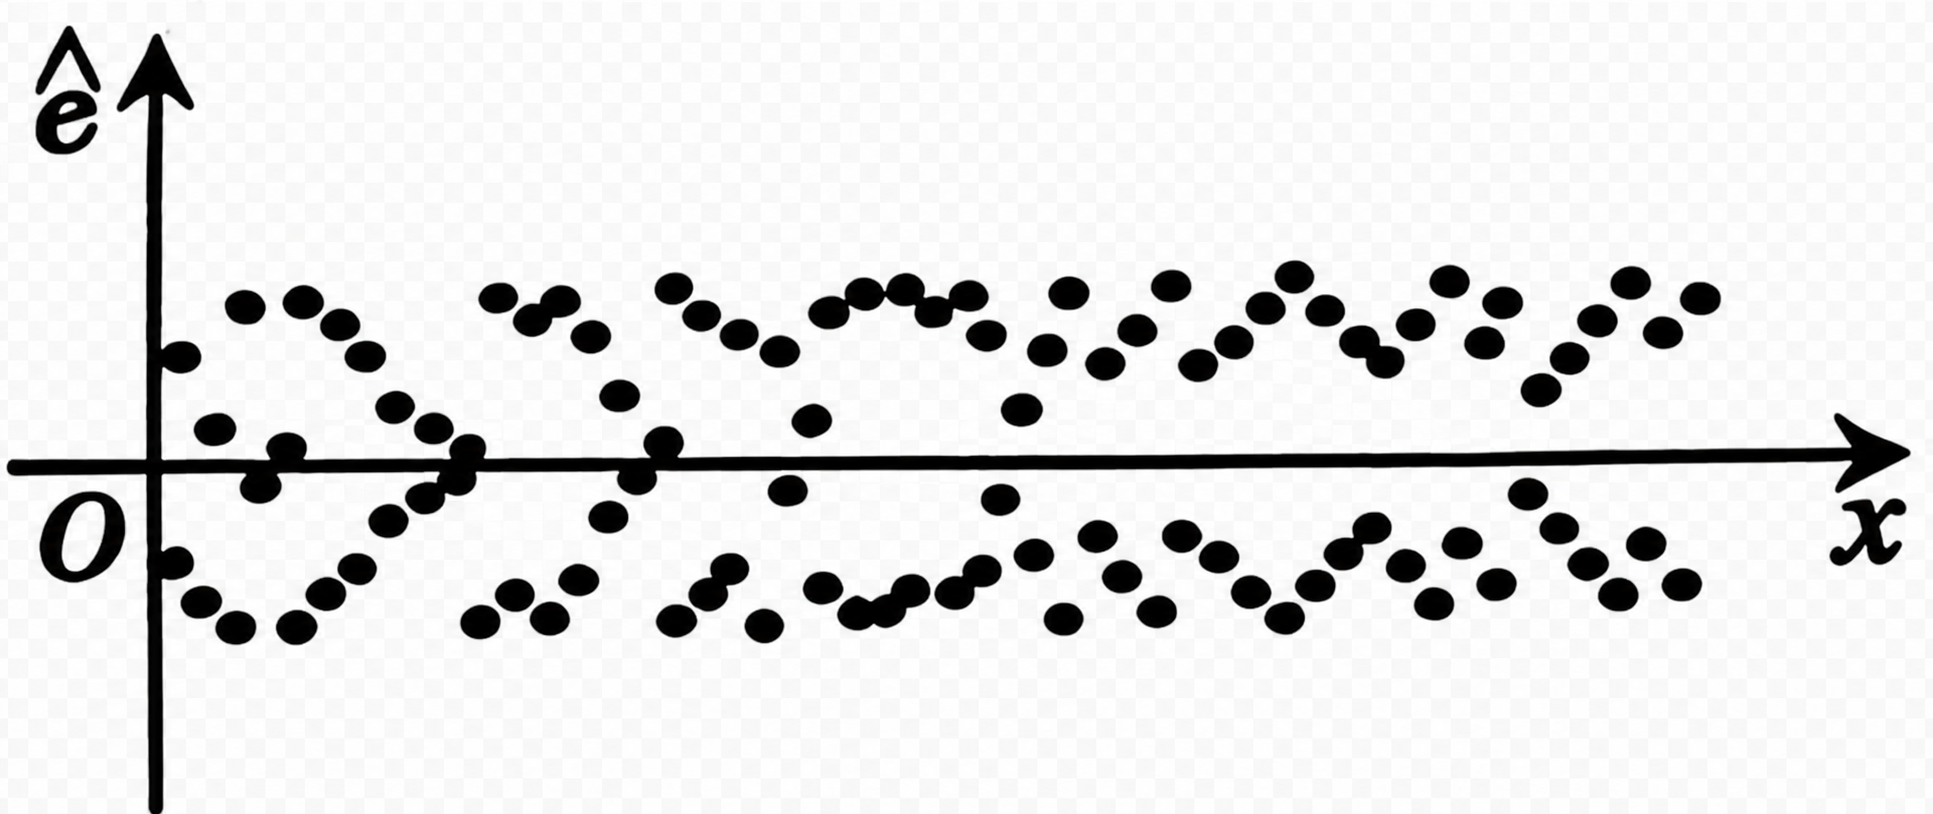
\includegraphics[width=\textwidth]{images/65cc2935ceea6efd236f015efc8d3c9744e38f4fa51f8e825f8ef97d83b9301c.png}\\
{\small 图 1}
\end{minipage}
\hfill
\begin{minipage}[t]{0.46\textwidth}
\centering
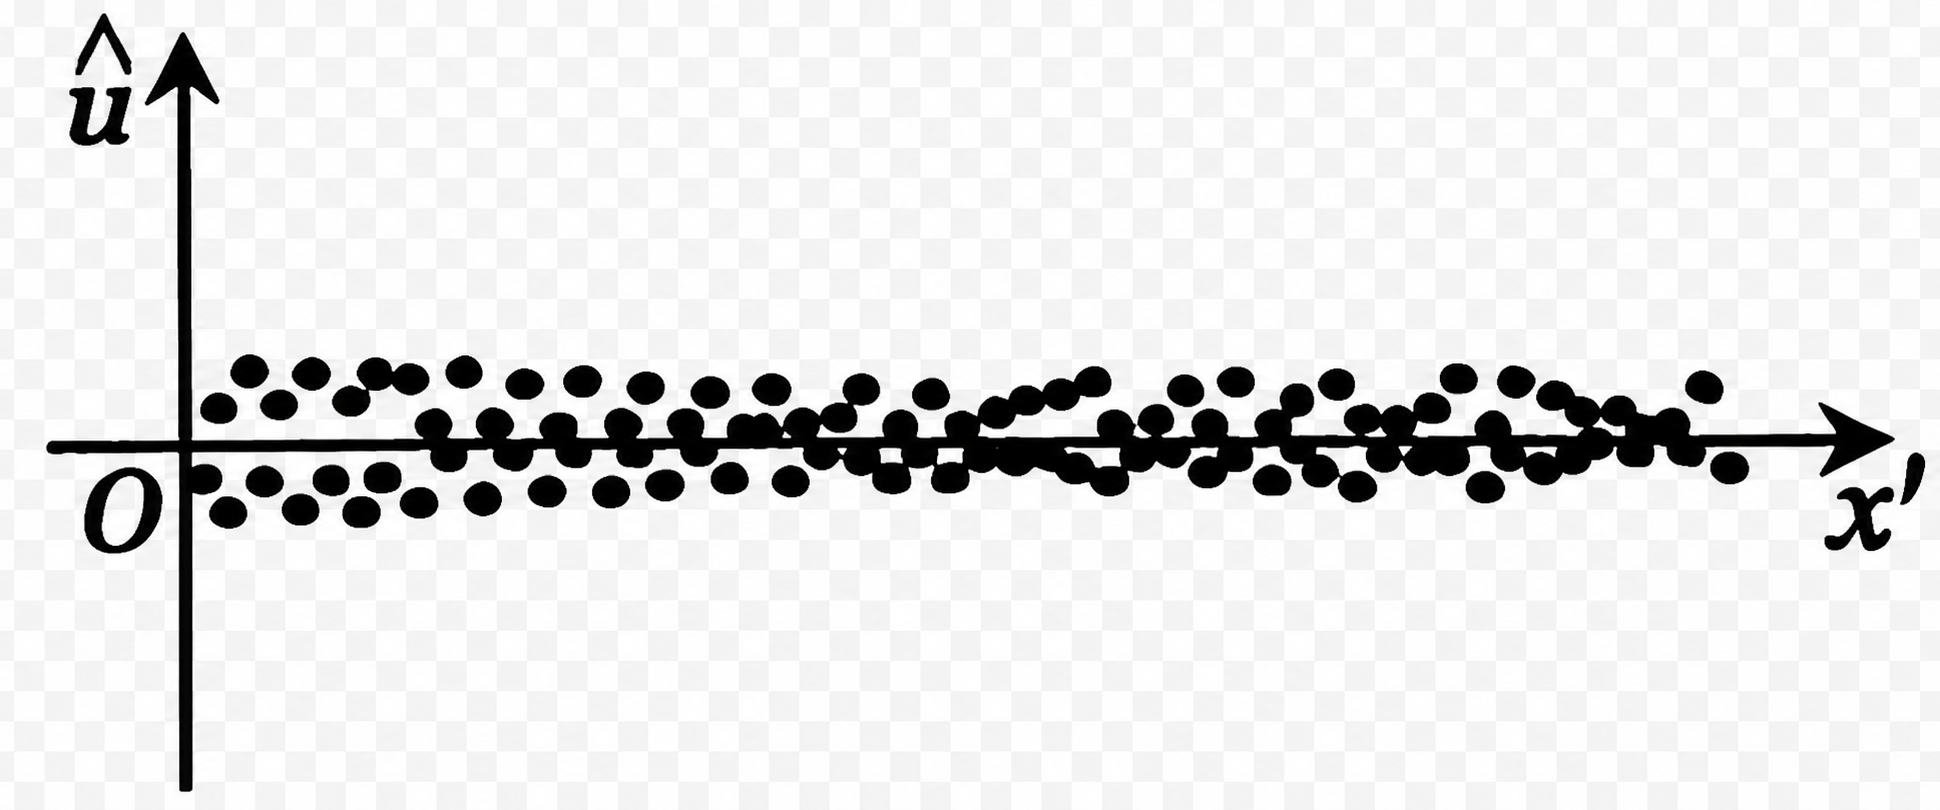
\includegraphics[width=\textwidth]{images/4a9eb6ac34ccbef48d752b747a94b80483b43a7809107c2f8a3a795e35f45a31.png}\\
{\small 图 2}
\end{minipage}
\end{center}

\vspace{2pt}
{\hspace{1.5em} A.\; 样本数据 $(x_{i}, y_{i})$ 负相关 \hfill
 B.\; $\hat{a}_{1} = 49.7$}

\vspace{1pt}
{\hspace{1.5em} C.\; $\sigma_{1}^{2} < \sigma_{2}^{2}$ \hfill
 D.\; 处理后的决定系数变大 \hspace{2em}}

\item 已知函数 $f(x) = \ln x - \cos x$，将 $f(x)$ 的所有极值点按照由小到大的顺序排列，得到数列 $\{x_{n}\}$，对于正整数 $n$，则下列说法中正确的有

\vspace{1pt}
{\hspace{1.5em} A.\; $\bigl(n - \frac{1}{2}\bigr)\pi < x_{n} < \bigl(n + \frac{1}{2}\bigr)\pi$ \hfill
 B.\; $x_{n+1} - x_{n} < \pi$}

\vspace{1pt}
{\hspace{1.5em} C.\; $\{\,|x_{n} - n\pi|\,\}$ 为递减数列 \hfill
 D.\; $f(x_{2n-1}) > \ln \dfrac{(4n-1)\pi}{2}$ \hspace{2em}}

\end{enumerate}


% ==================== 三、填空题 ====================
\section*{三、填空题：本题共 3 小题，每小题 5 分，共 15 分．}

\begin{enumerate}[leftmargin=2em,itemsep=10pt,resume]

\item 记 $S_{n}$ 为等差数列 $\{a_{n}\}$ 的前 $n$ 项和，若 $a_{1} = -3$，$a_{5} = 5$，则 $S_{6} = $ \underline{\hspace{3cm}}．

\item 袋中有 2 个红球、5 个白球，现随机不放回地逐个摸出．设 $X$ 为``首次出现某一种颜色的球被全部摸出''时所需的摸球次数，则 $X = 3$ 的概率为 \underline{\hspace{3cm}}．

\item 一个底面边长和侧棱长均为 4 的正三棱柱密闭容器 $ABC$--$A_{1}B_{1}C_{1}$，其中盛有一定体积的水，当底面 $ABC$ 水平放置时，水面高为 $\dfrac{15}{4}$．当侧面 $AA_{1}B_{1}B$ 水平放置时（如图），容器内的水形成新的几何体．若该几何体的所有顶点均在同一个球面上，则该球的表面积为 \underline{\hspace{3cm}}．

\begin{center}
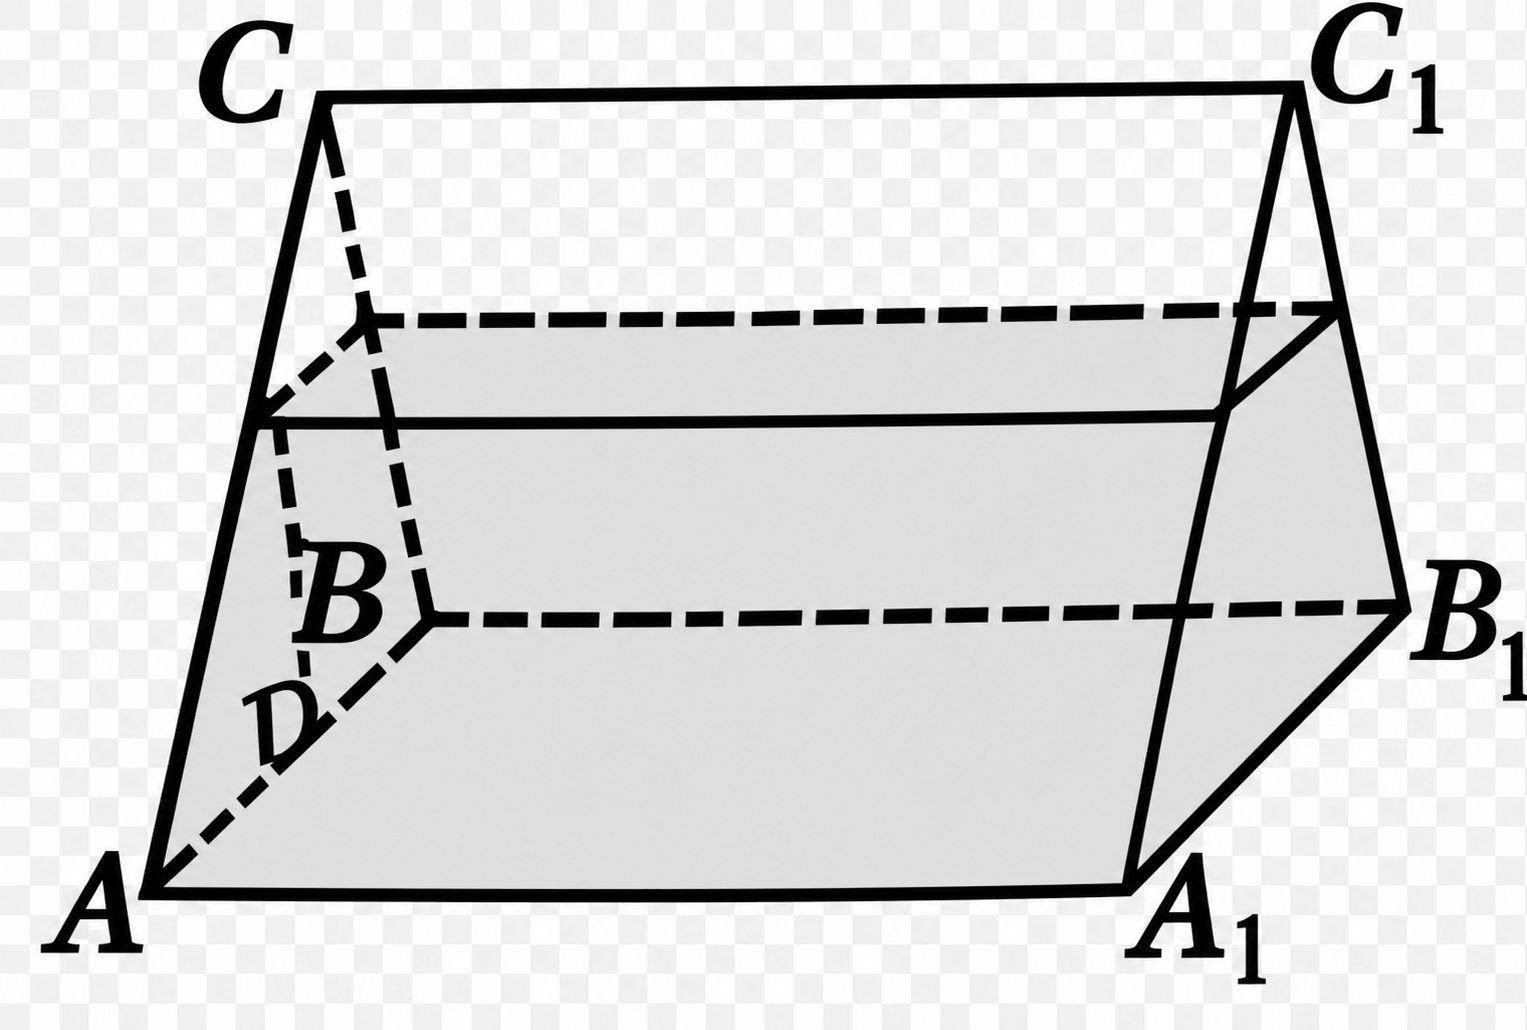
\includegraphics[width=0.42\textwidth]{images/6351f3f11ca38ff0b2fd31908714b961f3bab2eb31cfdc33b5a69bb708f975cd.png}
\end{center}

\end{enumerate}



% ==================== 四、解答题 ====================
\section*{四、解答题：本题共 5 小题，共 77 分．解答应写出文字说明、证明过程或演算步骤．}

\begin{enumerate}[leftmargin=2em,itemsep=6pt,resume]

% ---------- 第15题 ----------
\item （13 分）

某沙漠地区经过治理，生态系统得到很大改善，野生动物数量有所增加．为调查该地区某种野生动物的数量，将其分成面积相近的 200 个地块，从这些地块中用简单随机抽样的方法抽取 40 个作为样区，工作人员将区域内的地块按植被情况分为高覆盖地块、低覆盖地块两类，统计每块样区野生动物数量为``较多''或``较少''，统计结果如下：

\vspace{4pt}
\begin{center}
\begin{tabular}{lccc}
\toprule
& 高覆盖地块 & 低覆盖地块 & 合计 \\
\midrule
野生动物数量较多 & 14 &  6 & 20 \\
野生动物数量较少 &  8 & 12 & 20 \\
\midrule
合计 & 22 & 18 & 40 \\
\bottomrule
\end{tabular}
\end{center}

\begin{enumerate}[label=(\arabic*),leftmargin=3em,itemsep=3pt]
  \item 依据小概率值 $\alpha = 0.05$ 的独立性检验，判断是否有充分证据认为``该地区此种野生动物数量多少与地块植物覆盖面积高低存在关联'';
  \item 根据现有统计资料，各地块间植物覆盖面积差异很大．为提高样本的代表性以获得该地区这种野生动物数量更准确的估计，请给出一种你认为更合理的抽样方法，并说明理由．
\end{enumerate}

\vspace{6pt}
\begin{center}
\fbox{%
\begin{minipage}{0.92\textwidth}
\centering
\vspace{4pt}
$\displaystyle\chi^{2} = \frac{n(ad-bc)^{2}}{(a+b)(c+d)(a+c)(b+d)}$，其中 $n = a + b + c + d$
\vspace{4pt}
\end{minipage}%
}

\vspace{6pt}
\fbox{%
\begin{minipage}{0.92\textwidth}
\centering
\vspace{4pt}
\begin{tabular}{l|ccccc}
\toprule
$P(\chi^{2} \geqslant k_{\alpha})$ & 0.100 & 0.050 & 0.010 & 0.005 & 0.001 \\
\midrule
$k_{\alpha}$ & 2.706 & 3.841 & 6.635 & 7.879 & 10.828 \\
\bottomrule
\end{tabular}
\vspace{2pt}
\end{minipage}%
}
\end{center}

% ---------- 第16题 ----------
\item （15 分）

已知函数 $\displaystyle f(x) = \frac{a \cdot 3^{x} + 2}{3^{x} + 1} + x^{3}$，$a \in \mathbf{R}$．

\begin{enumerate}[label=(\arabic*),leftmargin=3em,itemsep=3pt]
  \item 当 $a = -2$ 时，求证：函数 $f(x)$ 是奇函数；
  \item 当 $a > -2$ 时，求 $\displaystyle f(1) + \frac{1}{f(-1)}$ 的最小值．
\end{enumerate}

% ---------- 第17题 ----------
\item （15 分）

在 $\triangle ABC$ 中，角 $A$、$B$、$C$ 的对边分别为 $a$、$b$、$c$，已知 $c = b \tan C$．

\begin{enumerate}[label=(\arabic*),leftmargin=3em,itemsep=3pt]
  \item 若 $B$ 为锐角，试判断 $\triangle ABC$ 的形状；
  \item 若 $B$ 为钝角，求 $\sin A + \sin C$ 的最大值．
\end{enumerate}


% ---------- 第18题 ----------
\item （17 分）

已知函数 $f(x) = a^{2}x^{2} - 3ax \ln x$，$a > 0$．

\begin{enumerate}[label=(\arabic*),leftmargin=3em,itemsep=3pt]
  \item 当 $a = 1$ 时，求曲线 $y = f(x)$ 在 $(1, f(1))$ 处的切线方程；
  \item 讨论 $f(x)$ 的零点个数；
  \item 当 $a > 2$ 时，证明：$f(x) > 2x$．
\end{enumerate}

% ---------- 第19题 ----------
\item （17 分）

某款游戏预推出一项皮肤抽卡活动，玩家每次抽卡需要花费 10 元，现有以下两种方案．方案一：没有保底机制，每次抽卡抽中新皮肤的概率为 $p_{1}$；方案二：每次抽卡抽中新皮肤的概率为 $p_{2}$，若连续 9 次未抽中，则第 10 次必中新皮肤．已知 $0 < p_{2} < p_{1} < 1$，玩家按照一、二两种方案进行抽卡，首次抽中新皮肤时的累计花费为 $X$，$Y$（元）．

\begin{enumerate}[label=(\arabic*),leftmargin=3em,itemsep=3pt]
  \item 按照方案一，小明先抽取三次，没有抽中皮肤，则他第四次抽中皮肤的概率是多少？
  \item 设第 $k$ 次首次抽中皮肤，求 $P(X = 10k)$，$P(Y = 10k)$；
  \item 若 $p_{1} = 2p_{2} = 0.1$，根据花费的均值从游戏策划角度选择收益较高的方案．（参考数据：$0.95^{9} \approx 0.63$，$0.95^{10} \approx 0.60$．）
\end{enumerate}

\end{enumerate}


% ==================== 参 考 答 案 部 分 ====================
\newpage
\thispagestyle{answerstyle}
\pagestyle{answerstyle}

\begin{center}
\vspace*{0.5cm}
{\zihao{-2}\heiti 数学参考答案}\\[0.3em]
{\zihao{5}\kaishu 2025---2026 学年度第二学期高二年级期末教学质量监测}
\end{center}

\vspace{0.3cm}
{\small\noindent\rule{\textwidth}{0.4pt}}
\vspace{0.5cm}

% ---- 一、选择题 ----
{\heiti 一、选择题}

\vspace{0.3cm}
\begin{center}
\begin{tabular}{c|cccccccc}
\toprule
题号 & 1 & 2 & 3 & 4 & 5 & 6 & 7 & 8 \\
\midrule
答案 & C & B & B & C & D & A & $6\sqrt{2}$\footnotemark & A \\
\bottomrule
\end{tabular}
\end{center}
\footnotetext{题面给出的四个选项中无匹配项，正确答案为 $6\sqrt{2}$．}

\vspace{0.5cm}

% ---- 二、选择题 ----
{\heiti 二、选择题}

\vspace{0.3cm}
\begin{center}
\begin{tabular}{c|ccc}
\toprule
题号 & 9 & 10 & 11 \\
\midrule
答案 & ACD & ABD & ACD \\
\bottomrule
\end{tabular}
\end{center}

\vspace{0.5cm}

% ---- 三、填空题 ----
{\heiti 三、填空题}

\vspace{0.3cm}
\begin{center}
\begin{tabular}{c|ccc}
\toprule
题号 & 12 & 13 & 14 \\
\midrule
答案 & $12$ & $\displaystyle\frac{2}{21}$ & $\displaystyle\frac{100\pi}{3}$ \\
\bottomrule
\end{tabular}
\end{center}

\vspace{0.5cm}
{\small\noindent\rule{\textwidth}{0.4pt}}
\vspace{0.3cm}

% ---- 四、解答题详解 ----
{\heiti 四、解答题}

% --- 15 ---
\vspace{0.4cm}
{\heiti 15．（13 分）}

\textbf{解：}

（1）由列联表可得
\[
\chi^{2} = \frac{40(14 \times 12 - 6 \times 8)^{2}}{20 \times 20 \times 22 \times 18}
        = \frac{40}{11} \approx 3.636.
\]

因为 $3.636 < 3.841 = k_{0.05}$，

所以依据小概率值 $\alpha = 0.05$ 的独立性检验，没有充分证据认为该地区此种野生动物数量多少与地块植物覆盖面积高低存在关联．

（2）可采用分层随机抽样：先按植物覆盖程度将全部地块分为高覆盖、低覆盖等层，再按各层地块数占总体的比例，在每层内进行简单随机抽样．这样能使覆盖状况不同的地块都得到合理代表，并在层内差异较小时降低估计量的方差，从而提高估计精度．

\vspace{0.2cm}
{\small\noindent\rule{\textwidth}{0.2pt}}

% --- 16 ---
\vspace{0.4cm}
{\heiti 16．（15 分）}

\textbf{解：}

（1）当 $a = -2$ 时，
\[
f(x) = \frac{-2 \cdot 3^{x} + 2}{3^{x} + 1} + x^{3}
     = \frac{2(1 - 3^{x})}{3^{x} + 1} + x^{3}.
\]

于是
\[
f(-x) = \frac{2(1 - 3^{-x})}{3^{-x} + 1} - x^{3}
      = \frac{2(3^{x} - 1)}{3^{x} + 1} - x^{3}
      = -\frac{2(1 - 3^{x})}{3^{x} + 1} - x^{3}
      = -f(x).
\]

函数的定义域为 $\mathbf{R}$，关于原点对称，故 $f(x)$ 是奇函数．

（2）令 $t = a + 2 > 0$．直接计算得
\[
f(1)  = \frac{3a + 2}{4} + 1 = \frac{3(a + 2)}{4} = \frac{3t}{4},
\qquad
f(-1) = \frac{a + 6}{4} - 1 = \frac{a + 2}{4} = \frac{t}{4}.
\]

所以
\[
f(1) + \frac{1}{f(-1)}
   = \frac{3t}{4} + \frac{4}{t}
   \geqslant 2\sqrt{\frac{3t}{4} \cdot \frac{4}{t}}
   = 2\sqrt{3}.
\]

当且仅当 $\displaystyle\frac{3t}{4} = \frac{4}{t}$，即 $t = \dfrac{4}{\sqrt{3}}$（$a = \dfrac{4}{\sqrt{3}} - 2$）时取等号．

因此最小值为 $2\sqrt{3}$．

\vspace{0.2cm}
{\small\noindent\rule{\textwidth}{0.2pt}}

% --- 17 ---
\vspace{0.4cm}
{\heiti 17．（15 分）}

\textbf{解：}

由正弦定理及 $c = b\tan C$，有
\[
\sin C = \sin B \tan C.
\]

因为 $\sin C > 0$，所以 $\cos C = \sin B$，从而 $C$ 为锐角．

（1）若 $B$ 为锐角，则 $\sin B = \cos\bigl(\frac{\pi}{2} - B\bigr)$，且 $B, C \in \bigl(0, \frac{\pi}{2}\bigr)$，故
\[
C = \frac{\pi}{2} - B,
\]
于是 $A = \dfrac{\pi}{2}$．因此 $\triangle ABC$ 是以 $A$ 为直角的直角三角形．

（2）若 $B$ 为钝角，则
\[
C = B - \frac{\pi}{2},\qquad
A = \pi - B - C = \frac{\pi}{2} - 2C,
\]
其中 $0 < C < \dfrac{\pi}{4}$．令 $u = \sin C$，则 $0 < u < \dfrac{\sqrt{2}}{2}$，并且
\begin{align*}
\sin A + \sin C &= \cos 2C + \sin C
                 = 1 - 2\sin^{2}C + \sin C \\
               &= 1 - 2u^{2} + u
                 = \frac{9}{8} - 2\Bigl(u - \frac{1}{4}\Bigr)^{2}
                 \leqslant \frac{9}{8}.
\end{align*}

当 $\sin C = \dfrac{1}{4}$ 时等号成立，故最大值为 $\dfrac{9}{8}$．

\vspace{0.2cm}
{\small\noindent\rule{\textwidth}{0.2pt}}

% --- 18 ---
\vspace{0.4cm}
{\heiti 18．（17 分）}

\textbf{解：}

函数定义域为 $(0, +\infty)$．

（1）当 $a = 1$ 时，$f(x) = x^{2} - 3x \ln x$，
\[
f'(x) = 2x - 3(\ln x + 1).
\]

所以 $f(1) = 1$，$f'(1) = -1$，切线方程为
\[
y - 1 = -(x - 1),
\]
即 $y = -x + 2$．

（2）因为 $x > 0$ 且 $a > 0$，所以
\[
f(x) = 0 \iff ax = 3\ln x \iff a = \frac{3\ln x}{x}.
\]

设 $g(x) = \dfrac{3\ln x}{x}$，则
\[
g'(x) = \frac{3(1 - \ln x)}{x^{2}}.
\]

函数 $g$ 在 $(0, e)$ 上单调递增，在 $(e, +\infty)$ 上单调递减，且 $g(e) = \dfrac{3}{e}$；又因 $a > 0$，零点只能位于 $x > 1$．因此：

\begin{center}
\begin{tabular}{cc}
\toprule
$a$ 的取值范围 & $f(x)$ 的零点个数 \\
\midrule
$0 < a < \dfrac{3}{e}$ & 两个零点 \\[3pt]
$a = \dfrac{3}{e}$ & 一个零点 $x = e$ \\[3pt]
$a > \dfrac{3}{e}$ & 没有零点 \\
\bottomrule
\end{tabular}
\end{center}

（3）要证 $f(x) > 2x$，只需证
\[
a^{2}x - 3a\ln x > 2.
\]

对固定的 $a > 2$，令 $h(x) = a^{2}x - 3a\ln x$．则
\[
h'(x) = a^{2} - \frac{3a}{x},
\]
故 $h$ 在 $x = \dfrac{3}{a}$ 处取得最小值
\[
h_{\min} = 3a - 3a\ln\frac{3}{a} = 3a\Bigl(1 + \ln\frac{a}{3}\Bigr).
\]

设 $H(a) = 3a\bigl(1 + \ln\frac{a}{3}\bigr)$．当 $a > 2$ 时，
\[
H'(a) = 3\Bigl(2 + \ln\frac{a}{3}\Bigr) > 0,
\]
所以
\[
H(a) > H(2) = 6\Bigl(1 + \ln\frac{2}{3}\Bigr) > 2.
\]

因此对任意 $x > 0$，均有 $f(x) > 2x$．

\vspace{0.2cm}
{\small\noindent\rule{\textwidth}{0.2pt}}

% --- 19 ---
\vspace{0.4cm}
{\heiti 19．（17 分）}

\textbf{解：}

（1）方案一中每次抽卡相互独立．前三次未抽中不改变第四次抽中的概率，因此所求概率为 $p_{1}$．

（2）对方案一，当 $k \geqslant 1$ 时，前 $k - 1$ 次均未抽中且第 $k$ 次抽中，故
\[
P(X = 10k) = (1 - p_{1})^{k-1} p_{1}.
\]

对方案二，首次抽中最迟发生在第 $10$ 次，因此
\[
P(Y = 10k) =
\begin{cases}
(1 - p_{2})^{k-1} p_{2}, & 1 \leqslant k \leqslant 9, \\[4pt]
(1 - p_{2})^{9},          & k = 10, \\[4pt]
0,                        & k > 10.
\end{cases}
\]

（3）由 $p_{1} = 0.1$，方案一首次抽中所需次数服从几何分布，故
\[
E(X) = 10 \cdot \frac{1}{p_{1}} = 100.
\]

由 $p_{2} = 0.05$，记方案二首次抽中所需次数为 $N$，则
\begin{align*}
E(N) &= \sum_{k=1}^{10} P(N \geqslant k)
      = \sum_{k=1}^{10} 0.95^{k-1} \\[4pt]
     &= \frac{1 - 0.95^{10}}{0.05}
      \approx \frac{1 - 0.60}{0.05}
      = 8,
\end{align*}
所以 $E(Y) = 10 E(N) \approx 80$．

从游戏策划角度，方案一的平均收入（$100$ 元）高于方案二（$\approx 80$ 元），因此应选择方案一．

\end{document}
